% Created by tikzDevice version 0.6.2-92-0ad2792 on 2013-11-14 18:58:53
% !TEX encoding = UTF-8 Unicode
\documentclass[12pt, mainfont = Minion,     mainscale = 1.0, sansfont = Myriad,     sansscale = MatchLowercase, monofont = Consolas,   monoscale = MatchLowercase, mathfont = MinionMath, mathscale = 1.0]{mtikzfig}
\begin{document}

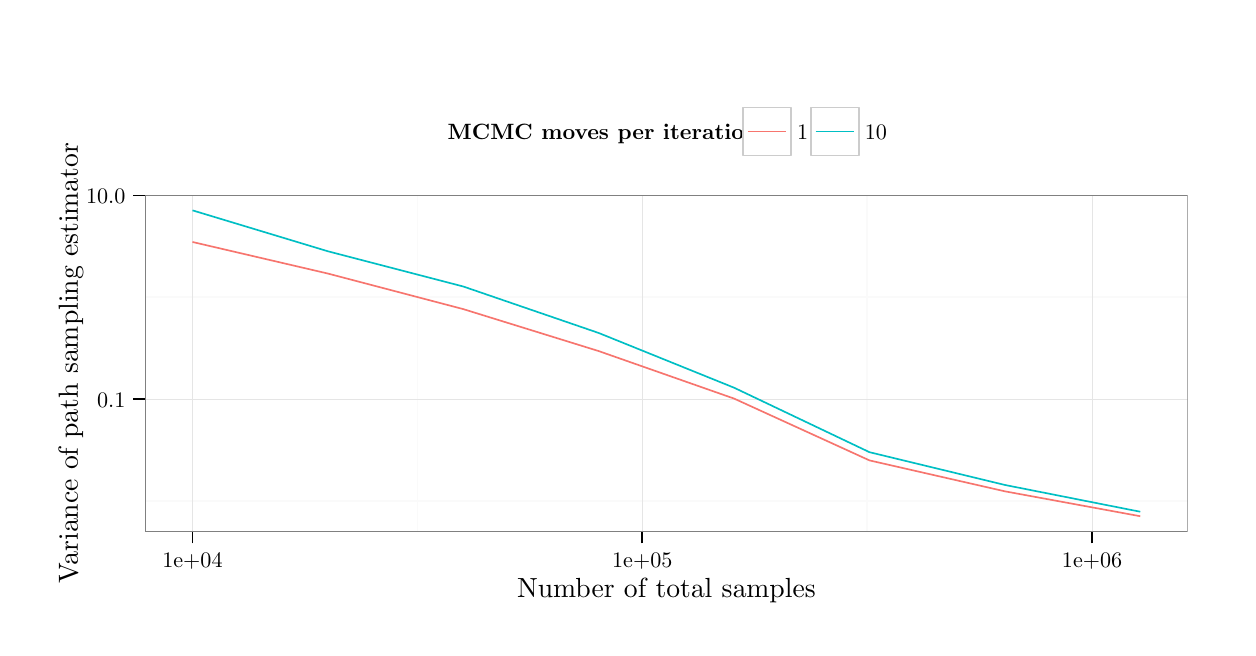
\begin{tikzpicture}[x=1pt,y=1pt]
\definecolor[named]{fillColor}{rgb}{1.00,1.00,1.00}
\path[use as bounding box,fill=fillColor,fill opacity=0.00] (0,0) rectangle (433.62,216.81);
\begin{scope}
\path[clip] (  0.00,  0.00) rectangle (433.62,216.81);
\definecolor[named]{drawColor}{rgb}{1.00,1.00,1.00}
\definecolor[named]{fillColor}{rgb}{1.00,1.00,1.00}

\path[draw=drawColor,line width= 0.6pt,line join=round,line cap=round,fill=fillColor] (  0.00,  0.00) rectangle (433.62,216.81);
\end{scope}
\begin{scope}
\path[clip] ( 42.43, 34.74) rectangle (419.17,156.33);
\definecolor[named]{fillColor}{rgb}{1.00,1.00,1.00}

\path[fill=fillColor] ( 42.43, 34.74) rectangle (419.17,156.33);
\definecolor[named]{drawColor}{rgb}{0.98,0.98,0.98}

\path[draw=drawColor,line width= 0.6pt,line join=round] ( 42.43, 45.86) --
	(419.17, 45.86);

\path[draw=drawColor,line width= 0.6pt,line join=round] ( 42.43,119.43) --
	(419.17,119.43);

\path[draw=drawColor,line width= 0.6pt,line join=round] (140.82, 34.74) --
	(140.82,156.33);

\path[draw=drawColor,line width= 0.6pt,line join=round] (303.35, 34.74) --
	(303.35,156.33);
\definecolor[named]{drawColor}{rgb}{0.90,0.90,0.90}

\path[draw=drawColor,line width= 0.2pt,line join=round] ( 42.43, 82.65) --
	(419.17, 82.65);

\path[draw=drawColor,line width= 0.2pt,line join=round] ( 42.43,156.22) --
	(419.17,156.22);

\path[draw=drawColor,line width= 0.2pt,line join=round] ( 59.55, 34.74) --
	( 59.55,156.33);

\path[draw=drawColor,line width= 0.2pt,line join=round] (222.09, 34.74) --
	(222.09,156.33);

\path[draw=drawColor,line width= 0.2pt,line join=round] (384.62, 34.74) --
	(384.62,156.33);
\definecolor[named]{drawColor}{rgb}{0.97,0.46,0.43}

\path[draw=drawColor,line width= 0.6pt,line join=round] ( 59.55,139.37) --
	(108.48,127.96) --
	(157.41,115.11) --
	(206.33, 99.95) --
	(255.26, 82.78) --
	(304.19, 60.44) --
	(353.11, 49.27) --
	(402.04, 40.27);
\definecolor[named]{drawColor}{rgb}{0.00,0.75,0.77}

\path[draw=drawColor,line width= 0.6pt,line join=round] ( 59.55,150.80) --
	(108.48,136.01) --
	(157.41,123.28) --
	(206.33,106.49) --
	(255.26, 86.71) --
	(304.19, 63.41) --
	(353.11, 51.57) --
	(402.04, 41.89);
\definecolor[named]{drawColor}{rgb}{0.50,0.50,0.50}

\path[draw=drawColor,line width= 0.6pt,line join=round,line cap=round] ( 42.43, 34.74) rectangle (419.17,156.33);
\end{scope}
\begin{scope}
\path[clip] (  0.00,  0.00) rectangle (433.62,216.81);
\definecolor[named]{drawColor}{rgb}{0.00,0.00,0.00}

\node[text=drawColor,anchor=base east,inner sep=0pt, outer sep=0pt, scale=  0.80] at ( 35.32, 79.72) {0.1};

\node[text=drawColor,anchor=base east,inner sep=0pt, outer sep=0pt, scale=  0.80] at ( 35.32,153.29) {10.0};
\end{scope}
\begin{scope}
\path[clip] (  0.00,  0.00) rectangle (433.62,216.81);
\definecolor[named]{drawColor}{rgb}{0.00,0.00,0.00}

\path[draw=drawColor,line width= 0.6pt,line join=round] ( 38.16, 82.65) --
	( 42.43, 82.65);

\path[draw=drawColor,line width= 0.6pt,line join=round] ( 38.16,156.22) --
	( 42.43,156.22);
\end{scope}
\begin{scope}
\path[clip] (  0.00,  0.00) rectangle (433.62,216.81);
\definecolor[named]{drawColor}{rgb}{0.00,0.00,0.00}

\path[draw=drawColor,line width= 0.6pt,line join=round] ( 59.55, 30.47) --
	( 59.55, 34.74);

\path[draw=drawColor,line width= 0.6pt,line join=round] (222.09, 30.47) --
	(222.09, 34.74);

\path[draw=drawColor,line width= 0.6pt,line join=round] (384.62, 30.47) --
	(384.62, 34.74);
\end{scope}
\begin{scope}
\path[clip] (  0.00,  0.00) rectangle (433.62,216.81);
\definecolor[named]{drawColor}{rgb}{0.00,0.00,0.00}

\node[text=drawColor,anchor=base,inner sep=0pt, outer sep=0pt, scale=  0.80] at ( 59.55, 21.77) {1e+04};

\node[text=drawColor,anchor=base,inner sep=0pt, outer sep=0pt, scale=  0.80] at (222.09, 21.77) {1e+05};

\node[text=drawColor,anchor=base,inner sep=0pt, outer sep=0pt, scale=  0.80] at (384.62, 21.77) {1e+06};
\end{scope}
\begin{scope}
\path[clip] (  0.00,  0.00) rectangle (433.62,216.81);
\definecolor[named]{drawColor}{rgb}{0.00,0.00,0.00}

\node[text=drawColor,anchor=base,inner sep=0pt, outer sep=0pt, scale=  1.00] at (230.80, 10.84) {Number of total samples};
\end{scope}
\begin{scope}
\path[clip] (  0.00,  0.00) rectangle (433.62,216.81);
\definecolor[named]{drawColor}{rgb}{0.00,0.00,0.00}

\node[text=drawColor,rotate= 90.00,anchor=base,inner sep=0pt, outer sep=0pt, scale=  1.00] at ( 18.16, 95.54) {Variance of path sampling estimator};
\end{scope}
\begin{scope}
\path[clip] (  0.00,  0.00) rectangle (433.62,216.81);
\definecolor[named]{fillColor}{rgb}{1.00,1.00,1.00}

\path[fill=fillColor] (147.52,166.40) rectangle (314.07,192.28);
\end{scope}
\begin{scope}
\path[clip] (  0.00,  0.00) rectangle (433.62,216.81);
\definecolor[named]{drawColor}{rgb}{0.00,0.00,0.00}

\node[text=drawColor,anchor=base west,inner sep=0pt, outer sep=0pt, scale=  0.80] at (151.79,176.42) {\bfseries MCMC moves per iteration};
\end{scope}
\begin{scope}
\path[clip] (  0.00,  0.00) rectangle (433.62,216.81);
\definecolor[named]{drawColor}{rgb}{0.80,0.80,0.80}
\definecolor[named]{fillColor}{rgb}{1.00,1.00,1.00}

\path[draw=drawColor,line width= 0.6pt,line join=round,line cap=round,fill=fillColor] (258.49,170.67) rectangle (275.84,188.02);
\end{scope}
\begin{scope}
\path[clip] (  0.00,  0.00) rectangle (433.62,216.81);
\definecolor[named]{drawColor}{rgb}{0.97,0.46,0.43}

\path[draw=drawColor,line width= 0.6pt,line join=round] (260.23,179.34) -- (274.10,179.34);
\end{scope}
\begin{scope}
\path[clip] (  0.00,  0.00) rectangle (433.62,216.81);
\definecolor[named]{drawColor}{rgb}{0.80,0.80,0.80}
\definecolor[named]{fillColor}{rgb}{1.00,1.00,1.00}

\path[draw=drawColor,line width= 0.6pt,line join=round,line cap=round,fill=fillColor] (283.00,170.67) rectangle (300.35,188.02);
\end{scope}
\begin{scope}
\path[clip] (  0.00,  0.00) rectangle (433.62,216.81);
\definecolor[named]{drawColor}{rgb}{0.00,0.75,0.77}

\path[draw=drawColor,line width= 0.6pt,line join=round] (284.74,179.34) -- (298.62,179.34);
\end{scope}
\begin{scope}
\path[clip] (  0.00,  0.00) rectangle (433.62,216.81);
\definecolor[named]{drawColor}{rgb}{0.00,0.00,0.00}

\node[text=drawColor,anchor=base west,inner sep=0pt, outer sep=0pt, scale=  0.80] at (278.00,176.42) {1};
\end{scope}
\begin{scope}
\path[clip] (  0.00,  0.00) rectangle (433.62,216.81);
\definecolor[named]{drawColor}{rgb}{0.00,0.00,0.00}

\node[text=drawColor,anchor=base west,inner sep=0pt, outer sep=0pt, scale=  0.80] at (302.52,176.42) {10};
\end{scope}
\end{tikzpicture}

\end{document}
